\documentclass[hyperref, UTF8]{ctexart}
\usepackage{graphicx}
\usepackage{float}
\usepackage{amsmath}
\usepackage{amsfonts}
\usepackage{amssymb}
\usepackage{fontspec}
\usepackage{tikz}
\usepackage{booktabs}
\setmonofont{Consolas}
\setCJKmainfont{Noto Sans SC Regular}
\usetikzlibrary{shapes.geometric, arrows}
\tikzstyle{startstop} = [rectangle, rounded corners, minimum width=3cm, minimum height=1cm,text centered, draw=black, fill=red!30]
\tikzstyle{io} = [trapezium, trapezium left angle=70, trapezium right angle=110, minimum width=3cm, minimum height=1cm, text centered, draw=black, fill=blue!30]
\tikzstyle{process} = [rectangle, minimum width=3cm, minimum height=1cm, text centered, draw=black, fill=orange!30]
\tikzstyle{empty_process} = [rectangle, minimum width=3cm, minimum height=1cm, text centered, draw=none, fill=none]
\tikzstyle{decision} = [diamond, minimum width=3cm, minimum height=1cm, text centered, draw=black, fill=green!30]
\tikzstyle{arrow} = [thick,->,>=stealth]
\usepackage[a4paper, top=3cm, bottom=3cm, left=3cm, right=3cm]{geometry}
\usepackage{subcaption}
\usepackage{xcolor}
\usepackage{animate}
\usepackage{listings}
\lstset{
	keywordstyle=\color{blue!70},
	commentstyle=\color{red!50!green!50!blue!50},
	frame=shadowbox,
	rulesepcolor=\color{red!20!green!20!blue!20},
	tabsize=2,
	basicstyle=\ttfamily\small,
	numberstyle=\tiny,
	numbers=left,
	showstringspaces=false,
	breaklines=true,
	language=MATLAB
}
\hypersetup{
	colorlinks=true,
	bookmarks=true,
	bookmarksopen=true,
	pdftitle=遥感综合实验~遥感图像目标检测,
	pdfauthor=16020710017~蓝彧文,
	linkcolor=blue
}
\title{遥感综合实验实验报告\\遥感图像目标检测}
\author{蓝彧文~16020710017}
\begin{document}
	\maketitle
	\tableofcontents
	\newpage
	实验中使用的所有代码和数据可以在\\ \url{https://github.com/EwenLan/remote-sensing-library}获取。
	\section{实验七~二值检测结果}
	\subsection{实验目的}
理解遥感图像目标检测的概念,根据之前所完成的实验以及所学习的算法自主设计目标检测方法,完成遥感图像的目标检测。
\subsection{实验原理}
\subsubsection{目标检测的概念}
从大场景的遥感图像中检测出感兴趣的目标。例如舰船目标,车辆目标等。给出目标的位置信息,并在原始图像中标注出来检测出的目标,提供目标的切片图像,用于后续的目标识别。
\subsubsection{目标检测的一般流程}
\begin{figure}[H]
	\centering
	\begin{tikzpicture}[node distance=4cm]
	\node[process](original_rs_img){原始遥感图像};
	\node[process, right of=original_rs_img](binary_detection){二值检测结果图像};
	\node[process, right of=binary_detection](abstract_optional_objs){候选目标提取};
	\node[process,right of=abstract_optional_objs](remove_false_alert){虚警去除};
	
	\draw[->] (original_rs_img) -- (binary_detection);
	\draw[->] (binary_detection) -- (abstract_optional_objs);
	\draw[->] (abstract_optional_objs) -- (remove_false_alert);
	\end{tikzpicture}
\end{figure}
\subsubsection{二值检测结果}
通过设计目标检测算法,从原始的遥感图像得到一个输出图像,该图像与原始图像具有相同的大小,但是为一幅二值图像,其中值为1的点代表目标像素点,值为0的点代表非目标像素点。
\begin{description}
	\item[目标检测的本质] 寻找目标与周围背景的差异性,根据这个差异性寻找目标。
	\item[一种可能的思路] 判断每一个像素点与它周围的背景像素点的差异性,如果差异性足够大,则该像素点判定为属于目标。
\end{description}
\subsubsection{目标检测的滑窗模型}
\begin{figure}[H]
	\centering
	\begin{tikzpicture}
	\filldraw[fill=blue!10] (0, 0) rectangle ++(5, 5) node[right] {背景窗};
	\filldraw[fill=yellow] (.5, .5) rectangle ++(4, 4) node[pos=0.8] {警戒窗};
	\filldraw[fill=lightgray] (2.25, 1.75) rectangle ++(2, 1) node[pos=0.8]{目标大小};
	\filldraw[fill=red] (2.25, 2.25) rectangle ++(.5, .5) node[pos=0.8, above]{当前检测的像素点};
	\end{tikzpicture}
\end{figure}
\subsection{实验流程}
\subsection{实验程序}
\subsection{实验结果和分析}
	\section{实验八~检测结果后处理}
	\subsection{实验目的}
理解遥感图像目标检测的概念,根据实验七中完成的实验数据,即二值检测结果,完成检测结果的后处理。包括连通分量提取与分析,目标像素聚类,以及目标切片的提取与显示等。
\subsection{实验原理}
\subsubsection{目标检测的一般流程}
\begin{figure}[H]
	\centering
	\begin{tikzpicture}[node distance=4cm]
	\node[process](raw_rs_img){原始遥感图像};
	\node[process, right of=raw_rs_img](binary_img){二值检测结果图像};
	\node[process, right of=binary_img](abstract_obj){候选目标提取};
	\node[process, right of=abstract_obj](remove_false_alert){虚警去除};
	
	\draw[->] (raw_rs_img) -- (binary_img);
	\draw[->] (binary_img) -- (abstract_obj);
	\draw[->] (abstract_obj) -- (remove_false_alert);
	\end{tikzpicture}
\end{figure}
\subsubsection{连通分量的提取}
\begin{figure}[H]
	\centering
	\begin{minipage}{0.45\linewidth}
		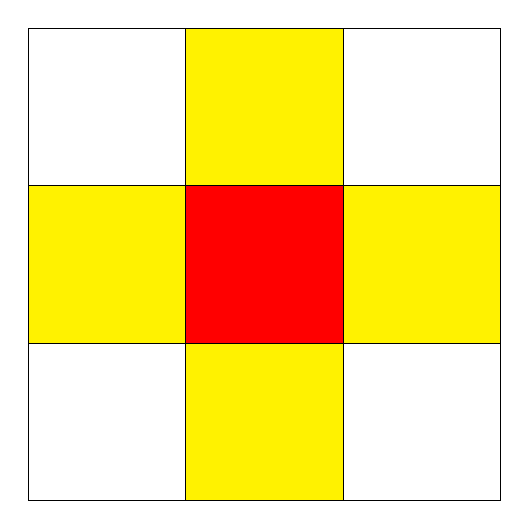
\begin{tikzpicture}
		\draw (0, 0) rectangle ++(6, 6);
		\filldraw[color=yellow, draw=black] (0, 2) rectangle ++(2, 2);
		\filldraw[color=yellow, draw=black] (2, 4) rectangle ++(2, 2);
		\filldraw[color=yellow, draw=black] (4, 2) rectangle ++(2, 2);
		\filldraw[color=yellow, draw=black] (2, 0) rectangle ++(2, 2);
		\filldraw (2, 2)[color=red, draw=black] rectangle ++(2, 2);
		\end{tikzpicture}
		\caption{四邻域}
	\end{minipage}
	\begin{minipage}{0.45\linewidth}
		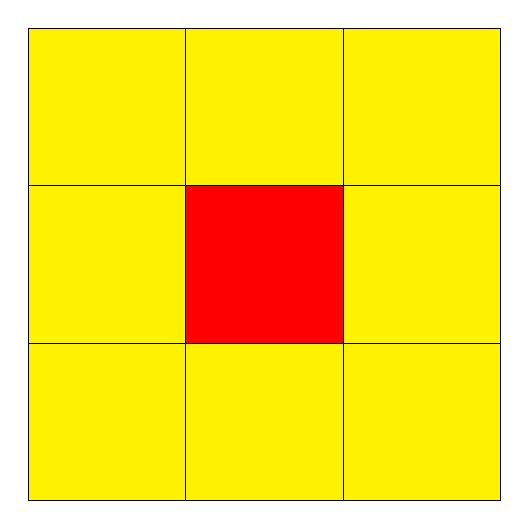
\begin{tikzpicture}
		\draw (0, 0) rectangle ++(6, 6);
		\filldraw (0, 0)[color=yellow, draw=black] rectangle ++(2, 2);
		\filldraw (0, 2)[color=yellow, draw=black] rectangle ++(2, 2);
		\filldraw (0, 4)[color=yellow, draw=black] rectangle ++(2, 2);
		\filldraw (2, 0)[color=yellow, draw=black] rectangle ++(2, 2);
		\filldraw (2, 2)[color=red, draw=black] rectangle ++(2, 2);
		\filldraw (2, 4)[color=yellow, draw=black] rectangle ++(2, 2);
		\filldraw (4, 0)[color=yellow, draw=black] rectangle ++(2, 2);
		\filldraw (4, 2)[color=yellow, draw=black] rectangle ++(2, 2);
		\filldraw (4, 4)[color=yellow, draw=black] rectangle ++(2, 2);
		\end{tikzpicture}
		\caption{八邻域}
	\end{minipage}
\end{figure}
\begin{description}
	\item[连通性] 两个像素是否连通取决于它们是否相邻以及它们的灰度值是否满足特定的相似性准则。
	\item[区域] 图像中的一个像素子集$\mathbb{R}$,该子集是一个连通集,则称$\mathbb{R}$为一个区域。
	\item[连通量] 具有相同输入值的邻接像素的区域。
	\item[连通分量的提取] 对每一个连通量,或每一个连通集$\mathbb{R}$赋予不同的标记。方便对$\mathbb{R}$进行分析。
	\item[$\mathbb{R}$的统计量] 面积,周长,质心,二阶矩等。最小外接矩形,$\mathbb{R}$区域的长度、宽度、长宽比。
\end{description}
\subsubsection{二值检测结果分析}
\begin{enumerate}
	\item 根据目标的大小,形状的先验知识,去除过大或过小的,形状不符合的连通区域。
	\item 对剩余的连通区域进行聚类,得到属于同一个目标的连通区域。
	\item 根据属于同一个目标的连通区域确定目标的中心。
	\item 以目标中心为中心切出目标候选切片。
	\item 进一步分析目标候选切片以去除虚警。
\end{enumerate}
连通区域聚类,得到属于同一个目标的连通区域。
\paragraph{层次聚类法}
\begin{enumerate}
	\item 每个连通区域自成一类,计算两辆距离,得到距离矩阵。
	\item 寻找距离最近的两个连通区域,划为一类。更新类别标记。
	\item 重新计算距离矩阵。
	\item 跳至步骤2,重复计算及合并。结束准则:最小距离大于一个阈值$T$。
\end{enumerate}
\subsection{实验流程}
\begin{figure}[H]
	\centering
	\begin{tikzpicture}[node distance=1.5cm]
	\node[startstop](begin){开始};
	\node[io, below of=begin](read_binarized_img){读取二值化判别图};
	\node[process, below of=read_binarized_img](label){标记连通区域};
	\node[process, below of=label](statistic){对连通区域计算质心、二阶矩};
	\node[process, below of=statistic](covariance){计算连通区域坐标协方差矩阵};
	\node[process, below of=covariance](area){计算连通区域面积};
	\node[process, below of=area](filte){筛选符合要求的目标};
	\node[process, below of=filte](mark_obj){在图片上标记目标};
	\node[io, below of=mark_obj](output){输出目标图像};
	\node[startstop, below of=output](end){结束};
	
	\draw[->] (begin) -- (read_binarized_img);
	\draw[->] (read_binarized_img) -- (label);
	\draw[->] (label) -- (statistic);
	\draw[->] (statistic) -- (covariance);
	\draw[->] (covariance) -- (area);
	\draw[->] (area) -- (filte);
	\draw[->] (filte) -- (mark_obj);
	\draw[->] (mark_obj) -- (output);
	\draw[->] (output) -- (end);
	\end{tikzpicture}
\end{figure}
\subsection{实验程序}
程序对不同连通分量的面积、质心、长宽比等参数进行计算,并依据面积和长宽比对目标进行筛选,以此筛选得到感兴趣对目标。
\lstinputlisting[caption={MarkBridge47.m}]{"../Executable Script/Exp 8/MarkBridge47.m"}
\lstinputlisting[caption={MarkBridge48.m}]{"../Executable Script/Exp 8/MarkBridge48.m"}
\lstinputlisting[caption={MarkBridge50.m}]{"../Executable Script/Exp 8/MarkBridge50.m"}
\lstinputlisting[caption={GetBinarizedImageObjectsInfo.m}]{"../Function Library/GetBinarizedImageObjectsInfo.m"}
\lstinputlisting[caption={DrawRectangle.m}]{"../Function Library/DrawRectangle.m"}
\lstinputlisting[caption={CutObjectsFromImage.m}]{"../Function Library/CutObjectsFromImage.m"}
\subsection{实验结果和分析}
\begin{figure}[H]
	\centering
	\begin{minipage}{0.45\linewidth}
		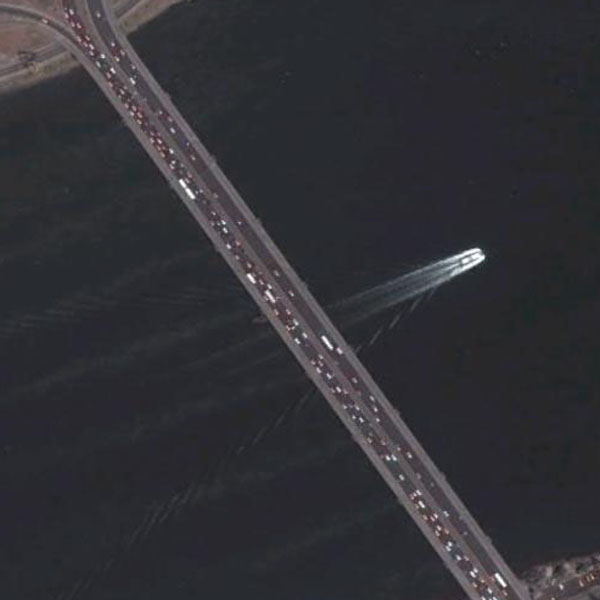
\includegraphics[width=\linewidth]{figure/bridge_47.jpg}
		\caption{bridge\_47原图}
	\end{minipage}
	\begin{minipage}{0.45\linewidth}
		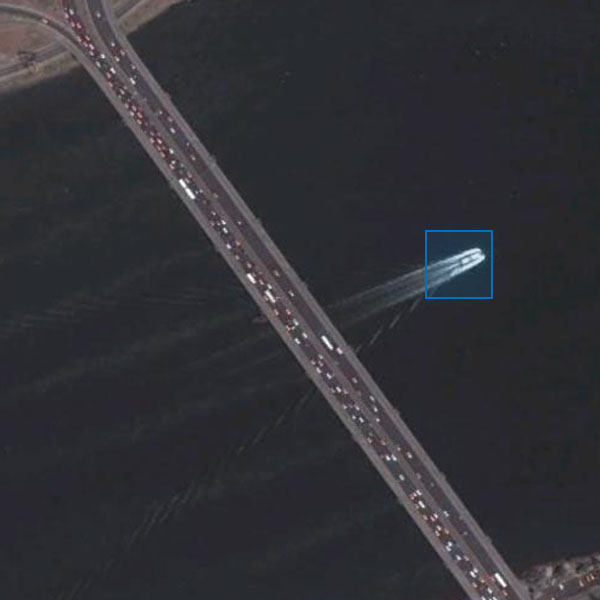
\includegraphics[width=\linewidth]{figure/bridge_47_marked_ship.png}
		\caption{bridge\_47检测结果}
	\end{minipage}
\end{figure}
\begin{figure}[H]
	\centering
	\begin{minipage}{0.45\linewidth}
		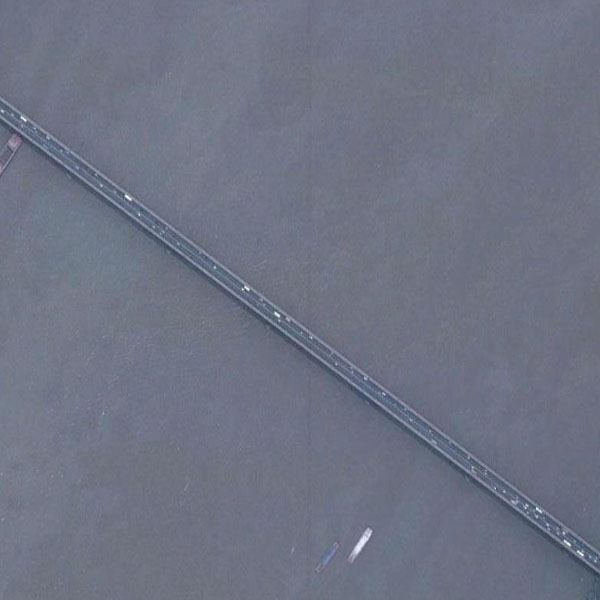
\includegraphics[width=\linewidth]{figure/bridge_48.jpg}
		\caption{bridge\_48原图}
	\end{minipage}
	\begin{minipage}{0.45\linewidth}
		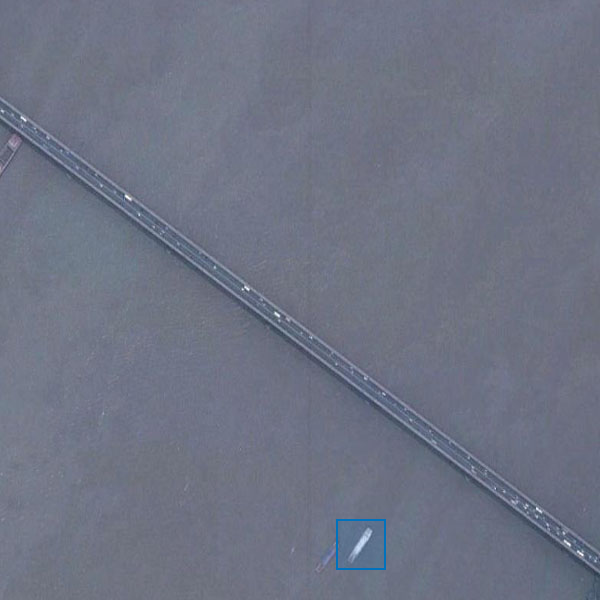
\includegraphics[width=\linewidth]{figure/bridge_48_marked_ship.png}
		\caption{bridge\_48检测结果}
	\end{minipage}
\end{figure}
\begin{figure}[H]
	\centering
	\begin{minipage}{0.45\linewidth}
		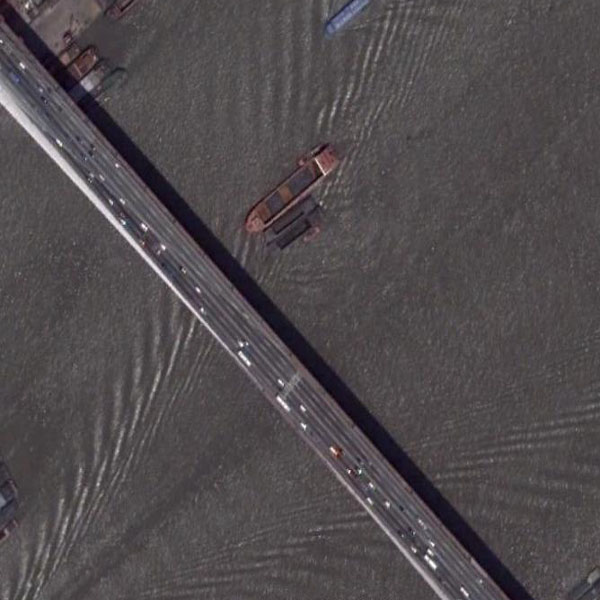
\includegraphics[width=\linewidth]{figure/bridge_50.jpg}
		\caption{bridge\_50原图}
	\end{minipage}
	\begin{minipage}{0.45\linewidth}
		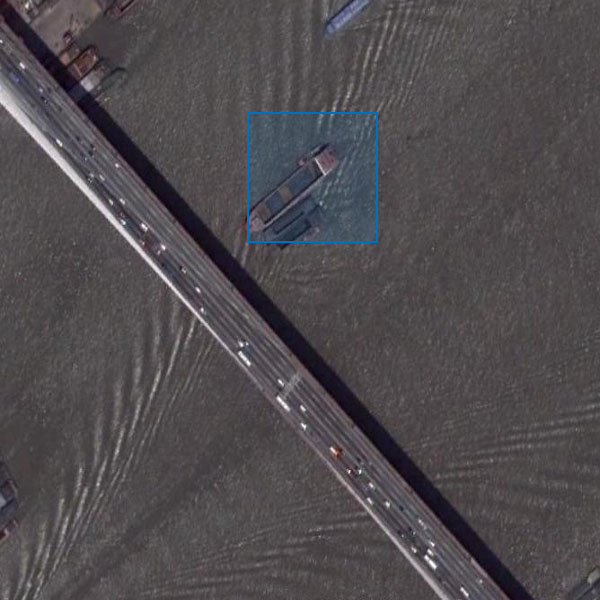
\includegraphics[width=\linewidth]{figure/bridge_50_marked_ship.png}
		\caption{bridge\_50检测结果}
	\end{minipage}
\end{figure}
\begin{figure}[H]
	\centering
	\begin{minipage}{0.3\linewidth}
		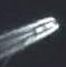
\includegraphics[width=\linewidth]{figure/bridge_47_cutted_object_1.png}
	\end{minipage}
	\begin{minipage}{0.3\linewidth}
		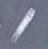
\includegraphics[width=\linewidth]{figure/bridge_48_cutted_object_1.png}
	\end{minipage}
	\begin{minipage}{0.3\linewidth}
		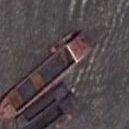
\includegraphics[width=\linewidth]{figure/bridge_50_cutted_object_1.png}
	\end{minipage}
	\caption{从图中截取的船只}
\end{figure}
对检测结果进行标记和筛选后,根据先验知识,我们可以设定筛选出船只的条件,比如面积、长宽比等特征。根据这些条件,我们可以从有许多虚警的图片中,筛选出最有可能是船只的目标。从上图可以看出,根据设定的筛选条件,程序成功的从图片中选出了图片中的船只。
	\section{实验九~传统目标识别方法}
	\subsection{实验目的}
理解遥感图像目标识别的概念,理解特征提取与分类的概念,学习主成分分析特征提取方法,以及K近邻分类方法,使用这两种方法完成目标识别。
\subsection{实验原理}
\subsubsection{目标识别的主要步骤}
\begin{figure}[H]
	\centering
	\begin{tikzpicture}[node distance=4cm]
	\node[process](rs_img){目标遥感图像};
	\node[process, right of=rs_img](abstract){特征提取};
	\node[process, right of=abstract](classifiler){分类器};
	\node[process, right of=classifiler](result){分类结果};
	
	\draw[->] (rs_img) -- (abstract);
	\draw[->] (abstract) -- (classifiler);
	\draw[->] (classifiler) -- (result);
	\end{tikzpicture}
\end{figure}
\subsubsection{特征提取}
由原始的观测数据得到变换后的用于分类的特征。变换的主要目的:
\begin{enumerate}
	\item 降低维数
	\item 提高类别可分性
\end{enumerate}
\[ \mathbf{Y}_m=\mathbf{A}_{m\times n}\mathbf{X}_n \]
\subsubsection{主成分分析}
\paragraph{最小重构误差准则}
\begin{description}
	\item[原始特征] $x_i\in \mathbb{R}^d,\quad i=1,2,\dots ,m$,均值为$0$。
	\item[特征变换的目的] 寻找一组新的坐标系$\left\lbrace w_1, w_2,\dots, w_d \right\rbrace$其中每一个向量为标准正交基。
	
	如果丢弃新坐标系中的部分坐标,将维度降低到$d'<d$,则样本在新坐标系中的投影为$\mathbf{z}_i=\left[ z_{i1}, z_{i2},\dots, z_{id} \right]$,重构向量为$\hat{x}_i=\sum_{i=1}^{d}z_{ij}w_j$,我们的目的是:
	$ \min\sum_{i=1}^{m}\left\| \hat{x}_i-x_i \right\|^2 $
	\item[上述问题的解] 样本协方差矩阵的前$d'$个最大的特征值对应的特征向量就是$\left\lbrace w_1, w_2,\dots,w_d \right\rbrace$。
	\item[计算过程]
	\begin{enumerate}
		\item 样本均值变为$0$。
		\item 计算样本协方差矩阵。
		\item 特征值分解,取最大特征值对应的特征向量。
		\item 得到投影矩阵$\mathbf{W}=\left[ w_1, w_2,\dots, w_d \right]$。
	\end{enumerate}
	\item[最大可分性原则] 投影后的向量为:$\mathbf{W}^\mathsf{T}x_i$。使得投影后的向量的方差最大化,推导的结果与前面等价。
	\item[$d'$的选择] $\frac{\sum_{i=1}^{d'}\lambda_i}{\sum_{i=1}^{d}\lambda_i}\leq l$
\end{description}
\paragraph{分类器}
\begin{description}
	\item[K近邻学习] 给定测试样本,基于某种距离度量找出训练样本集中与其最靠近的K个样本,基于K个近邻的信息来进行分类。可使用投票法完成分类,即K个近邻中出现最多的类别作为分类结果。
	 
	$K=1$时,成为最近邻分类器。
\end{description}
\paragraph{分类结果评价}
评价指标:分类准确率。
\subsection{实验流程}
\begin{figure}[H]
	\centering
	\begin{tikzpicture}[node distance=1.5cm]
	\node[startstop](begin){开始};
	\node[io, below of=begin](read_set){读取已标示的数据集};
	\node[process, below of=read_set](cut_img){分割数据集中的图片};
	\node[process, below of=cut_img](split_set){抽取训练样本和测试样本};
	\node[process, below of=split_set](pca){对所有样本进行PCA得到降维矩阵};
	\node[process, below of=pca](feature){对所有样本降维,得到特征向量};
	\node[process, below of=feature](classifying){对测试样本进行K近邻分类};
	\node[process, below of=classifying](accuracy){计算分类准确率};
	\node[io, below of=accuracy](output){输出分类准确率};
	\node[startstop, below of=output](end){结束};
	
	\draw[->] (begin) -- (read_set);
	\draw[->] (read_set) -- (cut_img);
	\draw[->] (cut_img) -- (split_set);
	\draw[->] (split_set) -- (pca);
	\draw[->] (pca) -- (feature);
	\draw[->] (feature) -- (classifying);
	\draw[->] (classifying) -- (accuracy);
	\draw[->] (accuracy) -- (output);
	\draw[->] (output) -- (end);
	\end{tikzpicture}
\end{figure}
\subsection{实验程序}
\lstinputlisting[caption={Images2Mat.m}]{"../Executable Script/Exp 9/Images2Mat2.m"}
\lstinputlisting[caption={CalculatePCAMat.m}]{"../Executable Script/Exp 9/CalculatePCAMat2.m"}
\lstinputlisting[caption={SplitDataSet.m}]{"../Executable Script/Exp 9/SplitDataSet2.m"}
\lstinputlisting[caption={TestClassifierPerformance.m}]{"../Executable Script/Exp 9/TestClassifierPerformence2.m"}
\lstinputlisting[caption={PrincipalComponentAnalysis.m}]{"../Function Library/PrincipalComponentAnalysis.m"}
\subsection{实验结果和分析}
使用上述程序,对原始的$600\times 600\times3$的森林、商业区、海滩和沙漠图片进行分割,成为$60\times 60\times 3$的小图片进行分类测试。

随机抽取不同类别的测试样本各1500个进行分类测试,可以得到如下表所示对分类结果。表中的每一行代表不同类别的测试样本,每一列代表不同类别的测试样本判断为这一分类的概率。所以,表中对角线上的概率即为这一分类的正确率。
\begin{center}
\begin{tabular}{ll|rrrr}
	\toprule
	&&\multicolumn{4}{c}{判定概率} \\
	 & & 森林 & 商业区 & 海滩 & 沙漠 \\
	 \midrule
	 \multirow{4}{*}{源数据类别} & 森林 & 91.93\% & 7.60\% & 0.33\% & 0.13\% \\
	  & 商业区 & 12.00\% & 84.80\% & 2.73\% & 0.47\% \\
	  & 海滩 & 1.07\% & 1.07\% & 96.40\% & 1.47\% \\
	  & 沙漠 & 0.07\% & 1.07\% & 0.13\% & 98.73\% \\
	 \bottomrule
\end{tabular}
\end{center}
由上表不难发现,从宏观上,使用主成分分析法和K近邻分类法对遥感图像进行分类可以取得比较优秀对分类结果,但仔细观察可以发现,对商业区的测试样本的分类还不太理想,对其他分类样本均有令人满意的分类结果。
\end{document}